%------------------------------------------------
\section{Background on epidemiological models}
%------------------------------------------------
\begin{frame}[t,label=abm_1]
	\frametitle{Background: epidemiological models}
	\tikzstyle{background grid}=[draw, black!50,step=.5cm]
	%
	What are compartmental epidemiological models?\\
	%
	\begin{columns}[t] % The "c" option specifies centered vertical alignment while the "t" option is used for top vertical alignment
		\begin{column}{.4\textwidth} % Left column and width
			\small
			\only<-6>{
				\begin{itemize}
					\uncover<2->{\item Described by a \emph{stochastic} process}%
					\uncover<4->{\item Assumes \emph{homogenous} interaction}
					\uncover<5->{\item Deterministic response for large $N$}
				\end{itemize}
				%
				\uncover<6->{
					\begin{equation*}
						\label{eq:SIRodes}
						\begin{aligned}
							&{\frac {dS}{dt}}=-{\frac {\beta IS}{N}},\\[6pt]
							&{\frac {dI}{dt}}={\frac {\beta IS}{N}}-\gamma I,\\[6pt]
							&{\frac {dR}{dt}}=\gamma I,
						\end{aligned}
					\end{equation*}
					{\scriptsize where $N = S + I + R$, $\beta$ controls infection spread, and $\gamma$ controls recovery rate}
				}%
			}%
			\only<7->{
				\begin{itemize}
					\item[\color{darkgreen} \ding{51}]<7-> Analytical solutions are available
					\item[\color{darkgreen} \ding{51}]<8-> Captures large-scale population dynamics
					\item[\color{red} \ding{56}]<9-> Does not account for \emph{geography}
					\item[\color{red} \ding{56}]<10-> Cannot model effect of intervention policies
				\end{itemize}
			}%
			%
		\end{column}
		%
		\begin{column}{.6\textwidth} % Left column and width

			\only<1>{
				\def\framel{1}
				\def\framep{1}
				\def\frameabm{1}
			}%
			\only<2>{
				\def\framel{1}
				\def\framep{2}
				\def\frameabm{1}
			}%
			\only<3>{
				\def\framel{1}
				\def\framep{2}
				\def\frameabm{1}
			}%
			\only<4-8>{
				\def\framel{1}
				\def\framep{2}
				\def\frameabm{2}
			}%
			\only<9->{
				\def\framel{1}
				\def\framep{2}
				\def\frameabm{3}
			}%

			\tikzstyle{background grid}=[draw, black!50,step=.1cm]
			\hspace*{5em}\raisebox{1em}{%
				\begin{tikzpicture}[scale=0.45, every node/.style={scale=0.45}, remember picture, overlay] %show background grid, 
						%%%%%%%%%%%%%%%%%%%%%%%%%%%%%%%%%%%%%%%%%%%%%%%%%%%%%%%%%
% preamble
\newcommand{\scolor}{blue!30}
\newcommand{\icolor}{red!30}
\newcommand{\rcolor}{black!30}
\newcommand{\fcolor}{black!70}
\newcommand{\legendshift}{-3}
%%%%%%%%%%%%%%%%%%%%%%%%%%%%%%%%%%%%%%%%%%%%%%%%%%%%%%%%%
\ifnum \framel = 1
    \renewcommand{\legendshift}{-0}
\else
    \renewcommand{\legendshift}{-3}
\fi
%
\node[circle, minimum size = 10mm, fill=blue!30] (S) at (0+\legendshift,-0) {\Large \color{black} \textit{S}};
\node[circle, minimum size = 10mm, fill=red!30] (I) at (4+\legendshift,-0) {\Large \color{black} \textit{I}};
\node[circle, minimum size = 10mm, fill=black!30] (R) at (8+\legendshift,-0) {\Large \color{black} \textit{R}};
\node[circle, minimum size = 10mm, fill=black!70] (F) at (12+\legendshift,-0) {\Large \color{white} \textit{F}};
%
\node[right, fill=white!70] at (S.east) {\Large susceptible};
\node[right, fill=white!70] at (I.east) {\Large infected};
\node[right, fill=white!70] at (R.east) {\Large recovered};
\node[right, fill=white!70] at (F.east) {\Large fatality};
%
\ifnum \framel > 1
    \node[diamond, minimum size = 12mm, fill=white!70, draw=black, line width=1 pt] (D) at (15+\legendshift,-0) {};
    \node[right, fill=white!70] at (D.east) {\Large random event};
\fi
						%%%%%%%%%%%%%%%%%%%%%%%%%%%%%%%%%%%%%%%%%%%%%%%%%%%%%%%%%
% preamble
\newcommand{\xshiftprocess}{0} 
\newcommand{\yshiftprocess}{-2} 
%%%%%%%%%%%%%%%%%%%%%%%%%%%%%%%%%%%%%%%%%%%%%%%%%%%%%%%%%
\ifnum \framep < 4
    \renewcommand{\yshiftprocess}{-3} 
\else
    \renewcommand{\yshiftprocess}{-2} 
\fi
%
\node[circle, minimum size = 15mm, fill=\scolor] (Ss) at (0+\xshiftprocess,-0+\yshiftprocess) {\LARGE \color{black} \textit{S}};
%
\ifnum \framep > 2
    \node[diamond, aspect=3, fill=white!70, draw=black, line width=1 pt] (contact) at (0+\xshiftprocess,-2.5+\yshiftprocess) {\LARGE made contact?};
    \node[circle, minimum size = 15mm, fill=\icolor] (Is) at (0+\xshiftprocess,-5+\yshiftprocess) {\Large \color{black} \textit{I}};
\else
    \node[circle, minimum size = 15mm, fill=\icolor] (Is) at (0+\xshiftprocess,-4+\yshiftprocess) {\Large \color{black} \textit{I}};
\fi
%
\ifnum \framep > 3
    \node[diamond, aspect=2, fill=white!70, draw=black, line width=1 pt] (hospital) at (0+\xshiftprocess,-7.5+\yshiftprocess) {\LARGE hospitalized?};
    \node[circle, minimum size = 15mm, fill=\rcolor] (Rs) at (-3+\xshiftprocess,-11+\yshiftprocess) {\Large \color{black} \textit{R}};
    \node[circle, minimum size = 15mm, fill=\fcolor] (Fs) at (3+\xshiftprocess,-11+\yshiftprocess) {\Large \color{white} \textit{F}};
\else
    \node[circle, minimum size = 15mm, fill=\rcolor] (Rs) at (-2+\xshiftprocess,-8+\yshiftprocess) {\Large \color{black} \textit{R}};
    \node[circle, minimum size = 15mm, fill=\fcolor] (Fs) at (2+\xshiftprocess,-8+\yshiftprocess) {\Large \color{white} \textit{F}};
\fi
%
\ifnum \framep > 1
    \path[-stealth,every node/.style={inner sep=2pt}]
        \ifnum \framep > 2
            (Ss) edge node [midway] {} (contact)
            (contact) edge node [left=0.1cm] {$P_\mathrm{I}$} (Is)
            {[out=0, in=0, looseness=2, fill=white] (Is) edge node [below=1cm] {$P_\mathrm{reinfect}$} (Ss)}
        \else
            (Ss) edge node [left=0.1cm] {$P_\mathrm{I}$} (Is)
            {[out=0, in=0, looseness=1] (Is) edge node [right=0.1cm] {$P_\mathrm{reinfect}$} (Ss)}
        \fi
        %
        \ifnum \framep > 3
            {[out=270, in=90] (Is.south) edge node {} (hospital.north)}
            %
            {[out=270, in=90] (hospital.south) edge node [below] {$P_{\mathrm{R}|h}$} (Rs.north)}
            {[out=270, in=90] (hospital.south) edge node [below] {$P_{\mathrm{F}|h}$} (Fs)}
            %
            {[out=180, in=90] (hospital.west) edge node [above left] {$P_{\mathrm{R}|h'}$} (Rs.north)}
            {[out=0, in=90] (hospital.east) edge node [above right] {$P_{\mathrm{F}|h'}$} (Fs)}
        \else
            {[out=270, in=90] (Is.south) edge node [above left] {$P_\mathrm{R}$} (Rs.north)}
            {[out=270, in=90] (Is) edge node [midway] [above right] {$P_\mathrm{F}$} (Fs)}
        \fi
    ;
\fi
						\only<3->{%%%%%%%%%%%%%%%%%%%%%%%%%%%%%%%%%%%%%%%%%%%%%%%%%%%%%%%%%
% preamble
\newif\ifS
\newif\ifI
\newif\ifR
\newif\ifF

\newcommand{\infectedlist}{2/4}
\newcommand{\recoveredlist}{2/3,5/5}
\newcommand{\fatalitylist}{3/2,5/1}

\newcommand{\depth}{5} 
\newcommand{\width}{5}  
\newcommand{\spacing}{2.3} 

\newcommand{\xshift}{4} 

\newcommand\IfStringInList[2]{\IfSubStr{,#2,}{,#1,}}

\newcommand{\circlecolor}{\scolor}
%%%%%%%%%%%%%%%%%%%%%%%%%%%%%%%%%%%%%%%%%%%%%%%%%%%%%%%%%
\ifnum \frameabm > 5
    \renewcommand{\recoveredlist}{1/3,2/3,3/3,3/4,3/5,5/5}
\fi

\foreach \i in {1,...,\width}
{
    % Input Layer
    \foreach \j in {1,...,\depth}
    {
        \IfStringInList{\i/\j}{\infectedlist}{\Itrue}{\Ifalse}
        \IfStringInList{\i/\j}{\recoveredlist}{\Rtrue}{\Rfalse}
        \IfStringInList{\i/\j}{\fatalitylist}{\Ftrue}{\Ffalse}
        
        \renewcommand{\circlecolor}{\scolor}
        
        \ifI
            \renewcommand{\circlecolor}{\icolor}
        \fi
        
        \ifR
            \renewcommand{\circlecolor}{\rcolor}
        \fi
        
        \ifF
            \renewcommand{\circlecolor}{\fcolor}
        \fi
            
        \node[circle, 
            minimum size = 10mm,
            fill=\circlecolor] (agent-\i\j) at (\xshift+ \i*\spacing,-\j*\spacing) {};
            
    }
    
}

 % Connect agents
\ifnum \frameabm > 1
    \foreach \i in {1,...,\width}
    {
        \foreach \j in {1,...,\depth}
        {
            \foreach \k in {1,...,\width}
            {
                \foreach \l in {1,...,\depth}
                {
                    
                    \IfSubStr{\i/\j}{\k/\l}{}{
                        
                        % heterogeneous interaction
                        \ifnum \frameabm > 3 
                            \pgfmathsetmacro{\distAB}{sqrt((\i-\k)^2 + (\j-\l)^2)}
                            \ifdim \distAB pt < 1.5 pt
                                
                                \ifnum \frameabm > 4
                                
                                    \IfStringInList{\i/\j}{\infectedlist}{
                                
                                        \IfStringInList{\k/\l}{\recoveredlist}{
                                        
                                            \draw[-, shorten >=1pt, opacity=0.2] (agent-\i\j) -- (agent-\k\l);
                                        }{
                                            \draw[-, color=red, line width=0.45 mm, shorten >=1pt, opacity=1.0] (agent-\i\j) -- (agent-\k\l);
                                        }
                                    }{
                                        \draw[-, shorten >=1pt, opacity=0.2] (agent-\i\j) -- (agent-\k\l);
                                    }
                                \else
                                    \draw[-, shorten >=1pt, opacity=0.4] (agent-\i\j) -- (agent-\k\l);
                                \fi
                                
                        \fi
                        \else
                            % homogeneous interaction
                            \IfStringInList{\i/\j}{\infectedlist}{
                                \ifnum \frameabm > 2
                                    \IfStringInList{\k/\l}{\recoveredlist}{
                                        \draw[-, shorten >=1pt, opacity=0.1] (agent-\i\j) -- (agent-\k\l);
                                    }{
                                        \draw[-, color=red, line width=0.45 mm, shorten >=1pt, opacity=1.0] (agent-\i\j) -- (agent-\k\l);
                                    }
                                \else
                                    \draw[-, shorten >=1pt, opacity=0.1] (agent-\i\j) -- (agent-\k\l);
                                \fi
                            }{
                                \draw[-, shorten >=1pt, opacity=0.1] (agent-\i\j) -- (agent-\k\l);
                            }
                        \fi
                    }
                }
            }
        }
    }
\fi}
				\end{tikzpicture}%
			}%
			\begin{tikzpicture}[remember picture, overlay] %show background grid, 
				\node [inner sep=0pt,above right, opacity=1.0]  at (-0.13\textwidth,-0.66\textheight) (seir) 
					{
						\only<6>{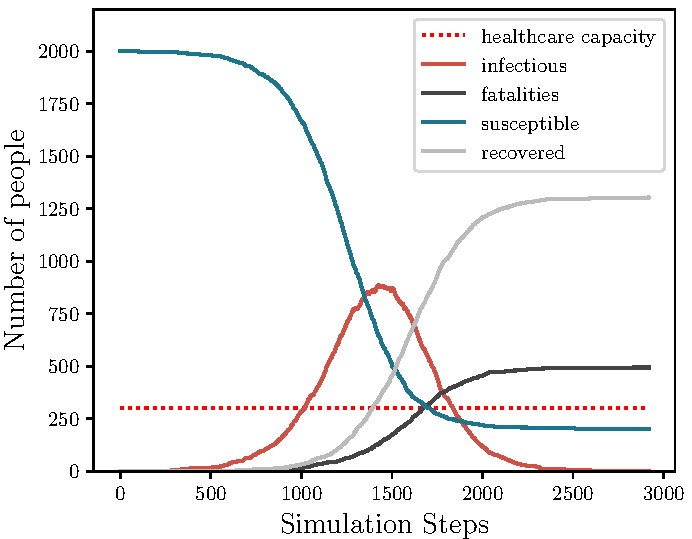
\includegraphics[width=0.9\textwidth]{SIR_example.pdf}}%
					};
			\end{tikzpicture}%
		\end{column}

	\end{columns}
	\vspace{-3em}
\end{frame}
%------------------------------------------------
\begin{frame}[t,label=abm_2]
	\frametitle{Background: epidemiological models}
	\tikzstyle{background grid}=[draw, black!50,step=.5cm]
	%
	What are agent-based epidemiological models?\\
	%
	\begin{columns}[t] % The "c" option specifies centered vertical alignment while the "t" option is used for top vertical alignment
		\begin{column}{.4\textwidth} % Left column and width
			\small
			\only<-12>{
				\begin{itemize}
					\uncover<2->{\item \emph{Stochastic} process}%
					\uncover<3->{\item Assume \emph{heterogenous} interaction}
					\uncover<5-12>{\item Stochastic response}
				\end{itemize}
			}%
			\only<13->{
				\begin{itemize}
					\item[\color{darkgreen} \ding{51}]<13-> Account for \emph{geography} and \emph{demographics}
					\item[\color{darkgreen} \ding{51}]<14-> Describe local phenomena
					\item[\color{darkgreen} \ding{51}]<15-> Can be used to model intervention policies
					\item[\color{red} \ding{56}]<16-> Stochastic response makes decision making challenging
					\item[\color{red} \ding{56}]<17-> Computationally expensive
				\end{itemize}
			}%
			%
		\end{column}
		%
		\begin{column}{.6\textwidth} % Left column and width

			\only<1>{
				\def\framel{1}
				\def\framep{2}
				\def\frameabm{1}
			}%
			\only<2>{
				\def\framel{2}
				\def\framep{3}
				\def\frameabm{1}
			}%
			\only<3>{
				\def\framel{2}
				\def\framep{3}
				\def\frameabm{4}
			}%
			\only<4-14>{
				\def\framel{2}
				\def\framep{3}
				\def\frameabm{5}
			}%
			\only<15->{
				\def\framel{2}
				\def\framep{4}
				\def\frameabm{6}
			}%
			\tikzstyle{background grid}=[draw, black!50,step=.1cm]
			\only<-4,13->{
				\hspace*{5em}\raisebox{1em}{%
					\begin{tikzpicture}[scale=0.45, every node/.style={scale=0.45}, remember picture, overlay] %show background grid, 
							%%%%%%%%%%%%%%%%%%%%%%%%%%%%%%%%%%%%%%%%%%%%%%%%%%%%%%%%%
% preamble
\newcommand{\scolor}{blue!30}
\newcommand{\icolor}{red!30}
\newcommand{\rcolor}{black!30}
\newcommand{\fcolor}{black!70}
\newcommand{\legendshift}{-3}
%%%%%%%%%%%%%%%%%%%%%%%%%%%%%%%%%%%%%%%%%%%%%%%%%%%%%%%%%
\ifnum \framel = 1
    \renewcommand{\legendshift}{-0}
\else
    \renewcommand{\legendshift}{-3}
\fi
%
\node[circle, minimum size = 10mm, fill=blue!30] (S) at (0+\legendshift,-0) {\Large \color{black} \textit{S}};
\node[circle, minimum size = 10mm, fill=red!30] (I) at (4+\legendshift,-0) {\Large \color{black} \textit{I}};
\node[circle, minimum size = 10mm, fill=black!30] (R) at (8+\legendshift,-0) {\Large \color{black} \textit{R}};
\node[circle, minimum size = 10mm, fill=black!70] (F) at (12+\legendshift,-0) {\Large \color{white} \textit{F}};
%
\node[right, fill=white!70] at (S.east) {\Large susceptible};
\node[right, fill=white!70] at (I.east) {\Large infected};
\node[right, fill=white!70] at (R.east) {\Large recovered};
\node[right, fill=white!70] at (F.east) {\Large fatality};
%
\ifnum \framel > 1
    \node[diamond, minimum size = 12mm, fill=white!70, draw=black, line width=1 pt] (D) at (15+\legendshift,-0) {};
    \node[right, fill=white!70] at (D.east) {\Large random event};
\fi
							%%%%%%%%%%%%%%%%%%%%%%%%%%%%%%%%%%%%%%%%%%%%%%%%%%%%%%%%%
% preamble
\newcommand{\xshiftprocess}{0} 
\newcommand{\yshiftprocess}{-2} 
%%%%%%%%%%%%%%%%%%%%%%%%%%%%%%%%%%%%%%%%%%%%%%%%%%%%%%%%%
\ifnum \framep < 4
    \renewcommand{\yshiftprocess}{-3} 
\else
    \renewcommand{\yshiftprocess}{-2} 
\fi
%
\node[circle, minimum size = 15mm, fill=\scolor] (Ss) at (0+\xshiftprocess,-0+\yshiftprocess) {\LARGE \color{black} \textit{S}};
%
\ifnum \framep > 2
    \node[diamond, aspect=3, fill=white!70, draw=black, line width=1 pt] (contact) at (0+\xshiftprocess,-2.5+\yshiftprocess) {\LARGE made contact?};
    \node[circle, minimum size = 15mm, fill=\icolor] (Is) at (0+\xshiftprocess,-5+\yshiftprocess) {\Large \color{black} \textit{I}};
\else
    \node[circle, minimum size = 15mm, fill=\icolor] (Is) at (0+\xshiftprocess,-4+\yshiftprocess) {\Large \color{black} \textit{I}};
\fi
%
\ifnum \framep > 3
    \node[diamond, aspect=2, fill=white!70, draw=black, line width=1 pt] (hospital) at (0+\xshiftprocess,-7.5+\yshiftprocess) {\LARGE hospitalized?};
    \node[circle, minimum size = 15mm, fill=\rcolor] (Rs) at (-3+\xshiftprocess,-11+\yshiftprocess) {\Large \color{black} \textit{R}};
    \node[circle, minimum size = 15mm, fill=\fcolor] (Fs) at (3+\xshiftprocess,-11+\yshiftprocess) {\Large \color{white} \textit{F}};
\else
    \node[circle, minimum size = 15mm, fill=\rcolor] (Rs) at (-2+\xshiftprocess,-8+\yshiftprocess) {\Large \color{black} \textit{R}};
    \node[circle, minimum size = 15mm, fill=\fcolor] (Fs) at (2+\xshiftprocess,-8+\yshiftprocess) {\Large \color{white} \textit{F}};
\fi
%
\ifnum \framep > 1
    \path[-stealth,every node/.style={inner sep=2pt}]
        \ifnum \framep > 2
            (Ss) edge node [midway] {} (contact)
            (contact) edge node [left=0.1cm] {$P_\mathrm{I}$} (Is)
            {[out=0, in=0, looseness=2, fill=white] (Is) edge node [below=1cm] {$P_\mathrm{reinfect}$} (Ss)}
        \else
            (Ss) edge node [left=0.1cm] {$P_\mathrm{I}$} (Is)
            {[out=0, in=0, looseness=1] (Is) edge node [right=0.1cm] {$P_\mathrm{reinfect}$} (Ss)}
        \fi
        %
        \ifnum \framep > 3
            {[out=270, in=90] (Is.south) edge node {} (hospital.north)}
            %
            {[out=270, in=90] (hospital.south) edge node [below] {$P_{\mathrm{R}|h}$} (Rs.north)}
            {[out=270, in=90] (hospital.south) edge node [below] {$P_{\mathrm{F}|h}$} (Fs)}
            %
            {[out=180, in=90] (hospital.west) edge node [above left] {$P_{\mathrm{R}|h'}$} (Rs.north)}
            {[out=0, in=90] (hospital.east) edge node [above right] {$P_{\mathrm{F}|h'}$} (Fs)}
        \else
            {[out=270, in=90] (Is.south) edge node [above left] {$P_\mathrm{R}$} (Rs.north)}
            {[out=270, in=90] (Is) edge node [midway] [above right] {$P_\mathrm{F}$} (Fs)}
        \fi
    ;
\fi
							%%%%%%%%%%%%%%%%%%%%%%%%%%%%%%%%%%%%%%%%%%%%%%%%%%%%%%%%%
% preamble
\newif\ifS
\newif\ifI
\newif\ifR
\newif\ifF

\newcommand{\infectedlist}{2/4}
\newcommand{\recoveredlist}{2/3,5/5}
\newcommand{\fatalitylist}{3/2,5/1}

\newcommand{\depth}{5} 
\newcommand{\width}{5}  
\newcommand{\spacing}{2.3} 

\newcommand{\xshift}{4} 

\newcommand\IfStringInList[2]{\IfSubStr{,#2,}{,#1,}}

\newcommand{\circlecolor}{\scolor}
%%%%%%%%%%%%%%%%%%%%%%%%%%%%%%%%%%%%%%%%%%%%%%%%%%%%%%%%%
\ifnum \frameabm > 5
    \renewcommand{\recoveredlist}{1/3,2/3,3/3,3/4,3/5,5/5}
\fi

\foreach \i in {1,...,\width}
{
    % Input Layer
    \foreach \j in {1,...,\depth}
    {
        \IfStringInList{\i/\j}{\infectedlist}{\Itrue}{\Ifalse}
        \IfStringInList{\i/\j}{\recoveredlist}{\Rtrue}{\Rfalse}
        \IfStringInList{\i/\j}{\fatalitylist}{\Ftrue}{\Ffalse}
        
        \renewcommand{\circlecolor}{\scolor}
        
        \ifI
            \renewcommand{\circlecolor}{\icolor}
        \fi
        
        \ifR
            \renewcommand{\circlecolor}{\rcolor}
        \fi
        
        \ifF
            \renewcommand{\circlecolor}{\fcolor}
        \fi
            
        \node[circle, 
            minimum size = 10mm,
            fill=\circlecolor] (agent-\i\j) at (\xshift+ \i*\spacing,-\j*\spacing) {};
            
    }
    
}

 % Connect agents
\ifnum \frameabm > 1
    \foreach \i in {1,...,\width}
    {
        \foreach \j in {1,...,\depth}
        {
            \foreach \k in {1,...,\width}
            {
                \foreach \l in {1,...,\depth}
                {
                    
                    \IfSubStr{\i/\j}{\k/\l}{}{
                        
                        % heterogeneous interaction
                        \ifnum \frameabm > 3 
                            \pgfmathsetmacro{\distAB}{sqrt((\i-\k)^2 + (\j-\l)^2)}
                            \ifdim \distAB pt < 1.5 pt
                                
                                \ifnum \frameabm > 4
                                
                                    \IfStringInList{\i/\j}{\infectedlist}{
                                
                                        \IfStringInList{\k/\l}{\recoveredlist}{
                                        
                                            \draw[-, shorten >=1pt, opacity=0.2] (agent-\i\j) -- (agent-\k\l);
                                        }{
                                            \draw[-, color=red, line width=0.45 mm, shorten >=1pt, opacity=1.0] (agent-\i\j) -- (agent-\k\l);
                                        }
                                    }{
                                        \draw[-, shorten >=1pt, opacity=0.2] (agent-\i\j) -- (agent-\k\l);
                                    }
                                \else
                                    \draw[-, shorten >=1pt, opacity=0.4] (agent-\i\j) -- (agent-\k\l);
                                \fi
                                
                        \fi
                        \else
                            % homogeneous interaction
                            \IfStringInList{\i/\j}{\infectedlist}{
                                \ifnum \frameabm > 2
                                    \IfStringInList{\k/\l}{\recoveredlist}{
                                        \draw[-, shorten >=1pt, opacity=0.1] (agent-\i\j) -- (agent-\k\l);
                                    }{
                                        \draw[-, color=red, line width=0.45 mm, shorten >=1pt, opacity=1.0] (agent-\i\j) -- (agent-\k\l);
                                    }
                                \else
                                    \draw[-, shorten >=1pt, opacity=0.1] (agent-\i\j) -- (agent-\k\l);
                                \fi
                            }{
                                \draw[-, shorten >=1pt, opacity=0.1] (agent-\i\j) -- (agent-\k\l);
                            }
                        \fi
                    }
                }
            }
        }
    }
\fi
					\end{tikzpicture}%
				}%
			}%
			%
			\begin{tikzpicture}[remember picture, overlay] %show background grid, 
				\node [inner sep=0pt,above right, opacity=1.0]  at (0.1\textwidth,-0.66\textheight) (abm) 
					{
						\only<5>{
							\begin{animateinline}[autoplay,width=0.9\textwidth]{60}
								\ifshowanimations
									\multiframe{77}{i=5+45}{%
										\includegraphics{render_demo_1_realization_1/sim_\i.pdf}
									}
								\else
									\multiframe{1}{i=3500+0}{%
										\includegraphics{render_demo_1_realization_1/sim_\i.pdf}
									}
								\fi
							\end{animateinline}%
						}%
						\only<6>{
							\begin{animateinline}[autoplay,width=0.9\textwidth]{60}
								\ifshowanimations
									\multiframe{77}{i=5+45}{%
										\includegraphics{render_demo_1_realization_2/sim_\i.pdf}
									}
								\else
									\multiframe{1}{i=3500+0}{%
										\includegraphics{render_demo_1_realization_2/sim_\i.pdf}
									}
								\fi
							\end{animateinline}%
						}%
					};
				\only<5>{\node[inner sep=0pt,align=flush center,above=\belowcaptionskip of abm,text width=\linewidth]
					{\vspace{-1em}{\large Realization 1}};}%
				\only<6>{\node[inner sep=0pt,align=flush center,above=\belowcaptionskip of abm,text width=\linewidth]
					{\vspace{-1em}{\large Realization 2}};}%
				%
				\node [inner sep=0pt,above right, opacity=1.0]  at (0.1\textwidth,-0.69\textheight) (trajectory) 
				{
					\only<7>{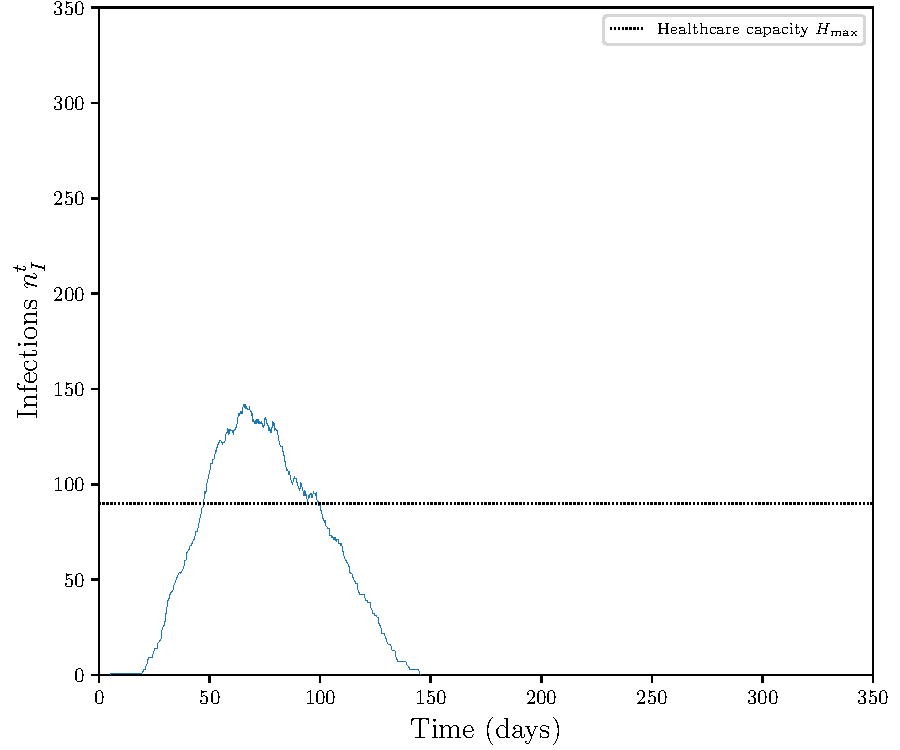
\includegraphics[width=0.85\textwidth]{realization_traces/I_compare_R_0.pdf}}%
					\only<8>{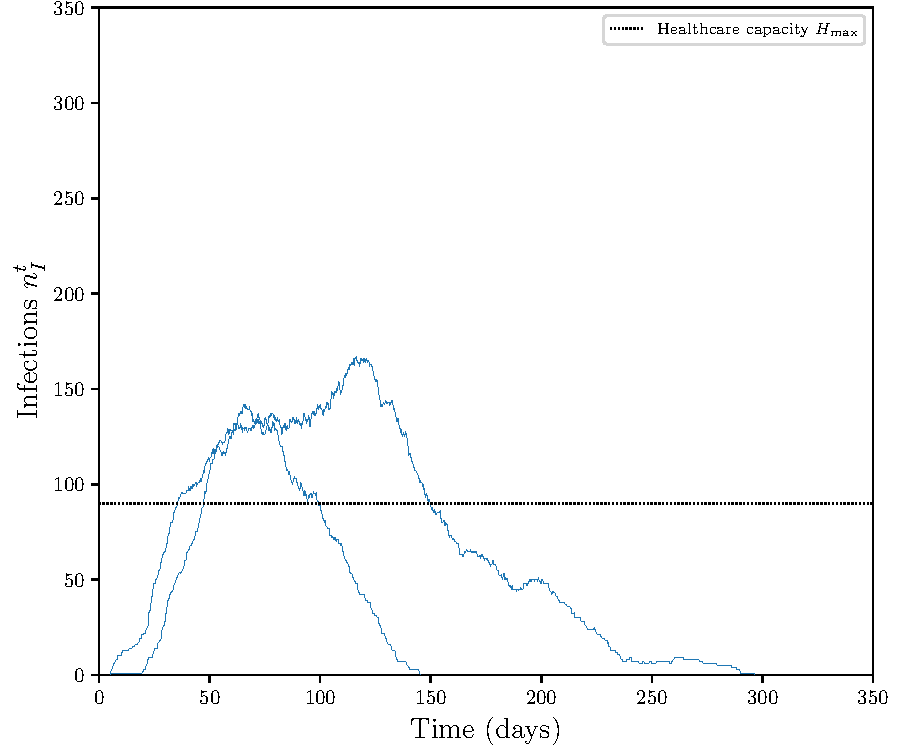
\includegraphics[width=0.85\textwidth]{realization_traces/I_compare_R_1.pdf}}%
					\only<9>{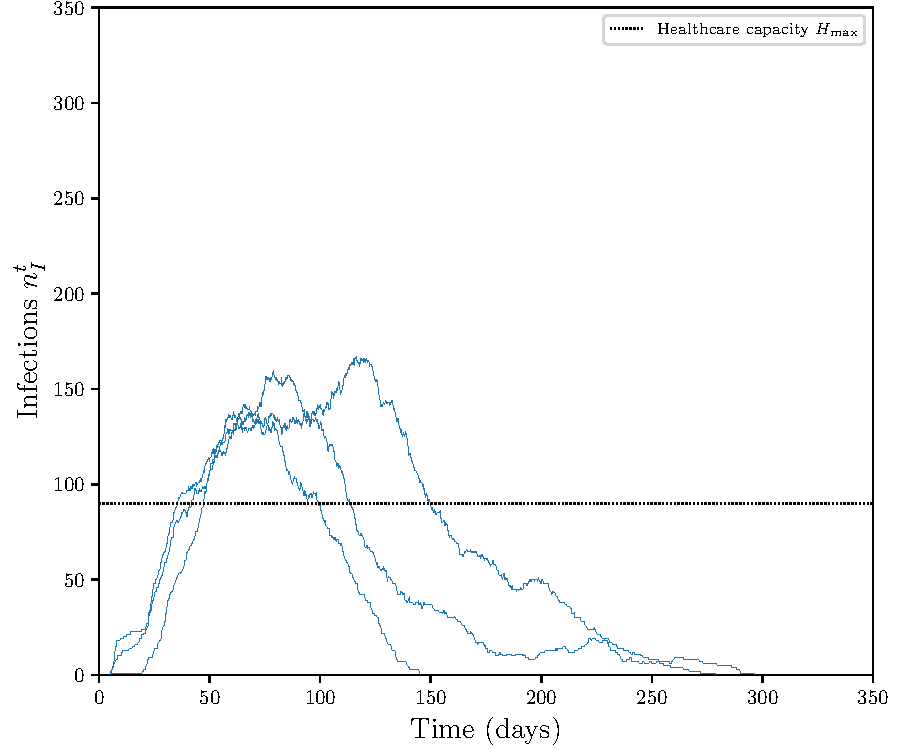
\includegraphics[width=0.85\textwidth]{realization_traces/I_compare_R_2.pdf}}%
					\only<10>{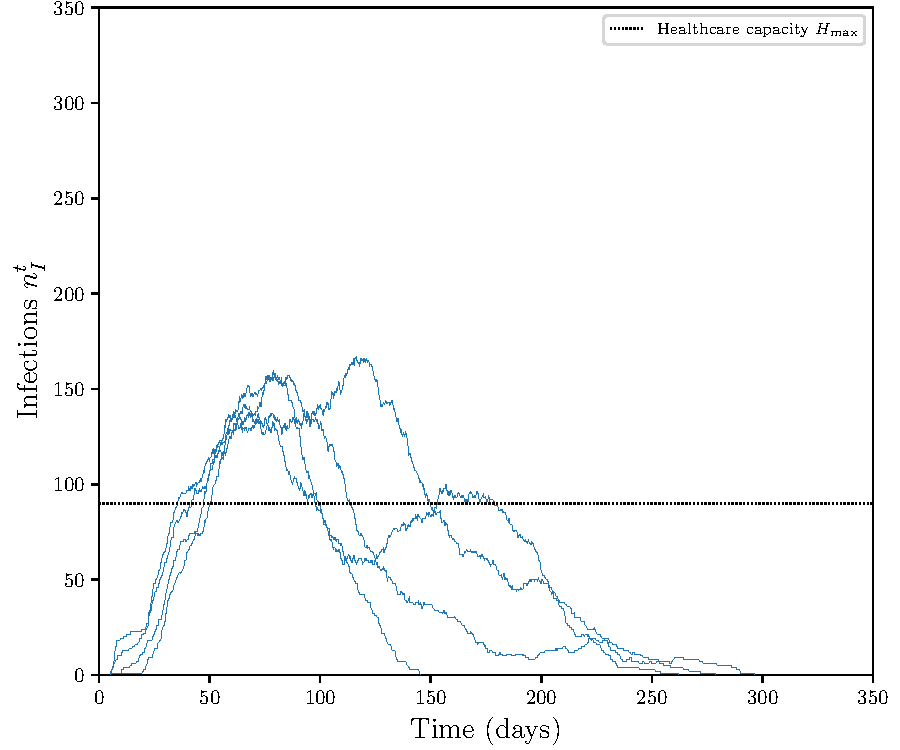
\includegraphics[width=0.85\textwidth]{realization_traces/I_compare_R_3.pdf}}%
					\only<11>{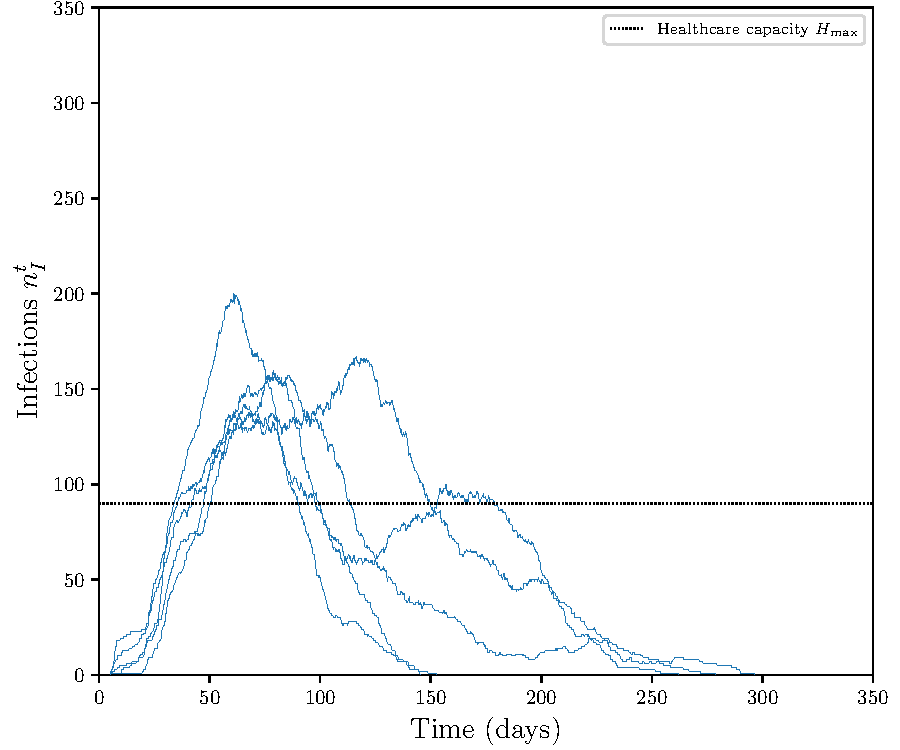
\includegraphics[width=0.85\textwidth]{realization_traces/I_compare_R_4.pdf}}%
					\only<12>{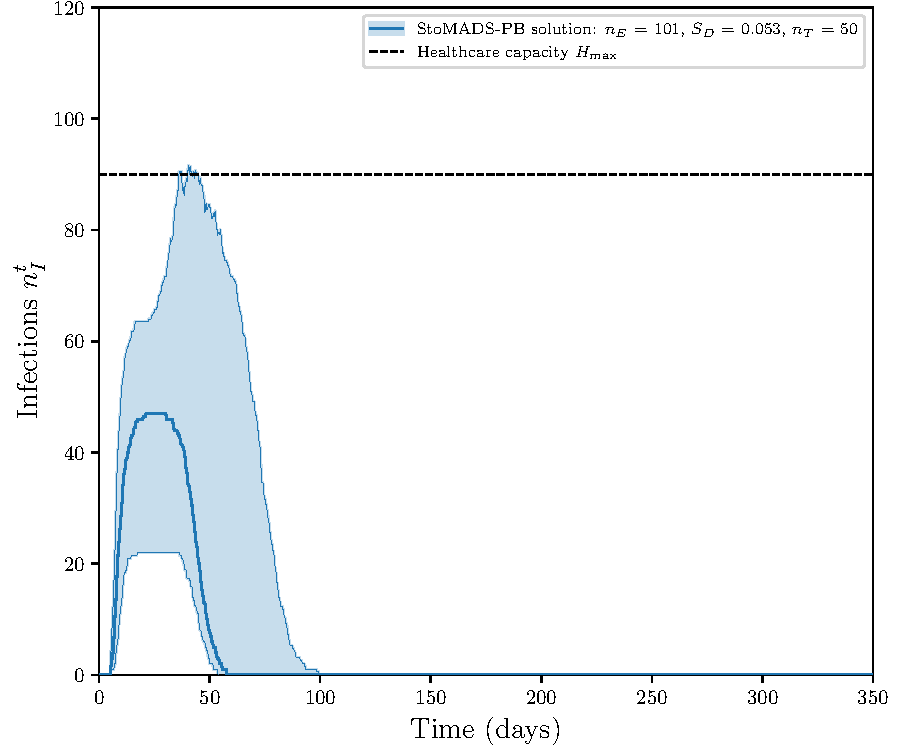
\includegraphics[width=0.85\textwidth]{realization_traces/I_compare_opt_0.pdf}}%
				};
				\only<7>{\node[inner sep=0pt,align=flush center,above=\belowcaptionskip of trajectory,text width=\linewidth]
					{\vspace{-1em}{\large Realization 1}};}%
				\only<8>{\node[inner sep=0pt,align=flush center,above=\belowcaptionskip of trajectory,text width=\linewidth]
					{\vspace{-1em}{\large Realization 2}};}%
			\end{tikzpicture}%
		\end{column}

	\end{columns}
	\vspace{-3em}
\end{frame}